\documentclass[12pt, a4paper, final]{report}

%Encoding
%--------------------------------------
\usepackage[utf8]{inputenc}
\usepackage[T1]{fontenc}
%--------------------------------------

%French-specific commands
%--------------------------------------
%\usepackage[frenchb]{babel}
\usepackage[autolanguage]{numprint}
%--------------------------------------

%Hyphenation rules
%--------------------------------------
%\usepackage{hyphenat}
%\hyphenation{mathéma-tiques récu-pérer}
%--------------------------------------

% Liens hypertext
%--------------------------------------
\usepackage{hyperref}

% Folder tree
%--------------------------------------
%\usepackage{dirtree}

%Other package
%--------------------------------------
\usepackage{titlesec} %titleformat
\usepackage{graphicx} %graphics
\usepackage{caption}
\usepackage{subcaption}
%--------------------------------------

%Disable "Chapter" before your chapter section
\titleformat{\chapter}[hang]{\bf\huge}{\thechapter}{2pc}{}

%%%%%%%%%%%%%%%%%%%%%%%%%%%%%%%%%%%%%%%%%%%%%

% Glossary
\usepackage[acronym]{glossaries}
\makeglossaries
\newglossaryentry{App}
{
    name={\textsc{App}}, 
    description={Application}
}

%%%%%%%%%%%%%%%%%%%%%%%%%%%%%%%%%%%%%%%%%%%%%

\begin{document}

%%%%%%%%%%%%%%%%%%%%%%%%%%%%%%%%%%%%%%%%%%%%%

\begin{titlepage}

    \centering
    
    
\includegraphics[width=0.75\textwidth]{./img/c00-main/logo.png}
    \par\vspace{1cm}
    {\scshape Hämeen ammattikorkeakoulu \\Hämeen ammattikorkeakoulu \par}
    \vspace{1cm}
    
    {\scshape\Large Project Report\par}
    \vspace{1.5cm}
    
    {\huge\bfseries Transportation modeling and Web content\par}
    \vspace{2cm}
    
    {\Large\itshape František Kolovský and Pierre-Vincent Vrot\par}
    \vfill
    
    Erasmus Exchange from \par
    \textsc{ZCU} ... \par
    \textsc{IMERIR} Institut Méditerranéen d’Étude et de Recherche en Informatique et Robotique \par

    \vfill
    
    {\large \today  \par version 0.1 \par}
    
\end{titlepage}

% Paragraphes spaces
%\setlength{\parindent}{4em}
\setlength{\parskip}{1em}
%\renewcommand{\baselinestretch}{1.5}

%%%%%%%%%%%%%%%%%%%%%%%%%%%%%%%%%%%%%%%%%%%%%

%Empty page
%--------------------------------------
\newpage
\null
\newpage

%%%%%%%%%%%%%%%%%%%%%%%%%%%%%%%%%%%%%%%%%%%%%

% INTRODUCTION
%--------------------------------------

\chapter*{Abstract}
\addcontentsline{toc}{chapter}{Abstract}
% ABSTRACT
%%%%%%%%%%%%%%%%%%%%%%%%%%%%%%%%%%%%%%%%%%%%%

% FRENCH
%%%%%%%%%%%%%%%%%%%%%%%%%%%%%%%%%%%%%%%%%%%%%

Les Systèmes d'Information Géographique (SIG) permettent, entre autres, d'acquérir, de traiter, d'organiser et de présenter des données géographiques, produisant ainsi des plans clairs, précis et intuitifs, et ce, à travers une composante web accessible depuis n'importe quel navigateur.

Le projet TraMap, proposé par HAMK et supervisé par Ramboll, est un outil simple et flexible permettant à un utilisateur de consulter des informations d'habitudes de transport issues de données géographiques en open source et d'en obtenir les informations sous forme d'application web et mobile.

C'est dans le cadre de ce besoin d'outil de consultation et d'exploitation des données que s'inscrit notre projet. Notre rôle est de rechercher des données open sources disponibles sur internet, d'en extraire les informations pour contruire un modèle d'habitude de transport, puis de développer une application de consultation des données multiplateformes. \\ \\

KEYWORDS
\par
\smallskip
\noindent \textbf{Keywords:} SIG, Modèle de Transport, Web, Algorithme, Sources Libres


\chapter*{Acknowledgments}
\addcontentsline{toc}{chapter}{Remerciements}
acknowledgments.tex

\setlength{\parskip}{0em}
\tableofcontents
\setlength{\parskip}{1em}

% MAIN
%--------------------------------------
\chapter*{Introduction}
\addcontentsline{toc}{chapter}{Introduction}
% Introduction
%%%%%%%%%%%%%%%%%%%%%%%%%%%%%%%%%%%%%%%%%%%%%

% FRENCH
%%%%%%%%%%%%%%%%%%%%%%%%%%%%%%%%%%%%%%%%%%%%%
Dans une Finlande où le vélo, la marche à pieds et les transports en communs sont de plus en plus utilisés, il devient nécessaire de se munir de moyens d'informations les plus utiles possibles afin de pouvoir anticiper les déplacements.

A l’ère actuelle, les entreprises sont toujours à l’affût de nouveautés, notamment dans le domaine SIG, que ce soit question de nouveaux outils ou de technologie. Chaque entreprises développent et commercialisent leurs outils d'information traffic. C'est dans une optique de partage de l'information, et du libre accès que va s'axer notre projet.

Aujourd'hui, open source et open data sont des sources d'information de plus en plus utilisées et permettent d'évoluer en communauté coopérative. Notre objectif principal, pour la réalisation de ce projet, est de récupérer les données et les outils open sources sur lesquels n'importe qui pourrait s'appuyer pour développer un modèle de consultation de données sur les habitudes de transport d'une ville. Notre cadre de recherche s'axera sur la ville de Hyvinkää et des données de déplacement à vélo.

Le travail réalisé se découpe en trois grandes parties : la première consiste à déterminer le modèle de transport théorique et mathématique des données qui seront consommées ; la seconde explique la façon dont une application peut être développée pour la consultation des données ; et enfin la troisième, et dernière partie, permet de combiner les précédentes parties afin d'obtenir un résultat consultable sur différentes plateformes.


\chapter{Transportation Modeling}
% TM - Theorical
%%%%%%%%%%%%%%%%%%%%%%%%%%%%%%%%%%%%%%%%%%%%%

%%%%%%%%%%%%%%%%%%%%%%%%%%%%%%%%%%%%%%%%%%%%%%%%%%%%%%%%%%%%%%%%%%%%%%%%%
% EN
%\section{Transportation model}

% FR
\section{Modèle de Transport}

% EN
%A transportation modelling is method for determining a traffic on road in focused area. Our goal is determine number of trip per road in road network from socio-economic and demographic data.

%Traditional transportation modelling have a several independent step (e.g trip generation, trip destination, ...). Our implementation of transportation modelling consist from 3 steps.

% FR
Un modèle de transport est une méthode déterminant un traffic sur les routes ciblé sur une zone décidée. Notre objectif est de déterminer un élément quantitatif d'afflux par route sur un réseau routier à partir de données socio-économiques et démographiques.

La modélisation de transport traditionnels possède plusieurs étape indépendantes (par exemple la génération de voyage, voyage destination, ...). Notre mise en oeuvre de la modélisation du transport se composent de 3 étapes :

% EN
% \begin{itemize}
%   \item[ ] \textbf{trip generation} - I this part we want to determine number of trip origin, destination in zones. This step is depend on data (e.g demographic data, socio-economic data, weather, local habits, ...). Quality of model depend a lot on these data.
%   \item[ ] \textbf{trip destination} - In this section we want determine \textit{transportation matrix} $T$ (OD matrix). It say how many people travel from zone $i$ to zone $j$. For it was used Gravity model.
%   \item[ ] \textbf{counting traffic} - This is last step.  We compute traffic for every road link (edge of graph).
% \end{itemize}

% FR
\begin{itemize}
  \item[ ] \textbf{la génération des déplacements} - Dans cette partie, nous voulons déterminer le nombre d'origine du voyage, la destination dans les zones. Cette étape est dépendent de données (par exemple des données démographiques, des données socio-économiques, météorologiques, les habitudes locales, ...). La qualité du modèle dépendra beaucoup de ces données.

  \item[ ] \textbf{la destination des déplacements} - Dans cette section nous voulons déterminer \textit{transportation matrix} $T$ (OD matrix). Cette matrice permet de dénombrer les  voyages entre une zone $i$ vers une zone $j$. Pour ce faire, nous utiliserons un modèle de gravité (Gravity Model).


  \item[ ] \textbf{Dénombrement du traffic} - Cette étape est la dernière. Nous calculons le trafic pour chaque liaison routière (bord du graphique).
\end{itemize}

% EN
%In upcoming section following expressions will be used:

% \begin{tabular}{ll}
%   $T$ & transportation matrix (number of trips between zones)\\
%   $C$ & travel cost matrix (between zones) \\
%   $T_i, T_j$ & sum value in row/column in $T$\\
%   $n$ & number of zones (size of matrix)
% \end{tabular}

% FR
Dans la suite de ce chapitre, les expressions suivantes vont être utilisées :

\begin{tabular}{ll}
  $T$ & transportation matrix (nombre de voyage entre deux zones)\\
  $C$ & travel cost matrix (le coup du voyage entre deux zones) \\
  $T_i, T_j$ & somme des valeurs en ligne/colonne dans $T$\\
  $n$ & nombre de zone (taille de la matrice)
\end{tabular}


%%%%%%%%%%%%%%%%%%%%%%%%%%%%%%%%%%%%%%%%%%%%%%%%%%%%%%%%%%%%%%%%%%%%%%%%%

% EN
%\subsection{Trip destination}

% FR
\subsection{Destinations des déplacements}

% EN
% For determine transportation matrix $T$ was used Gravity model:
% $$T_{ij} = K_i K_j T_i T_j f(C_{ij})$$
% where
% $$T_i = \sum_{j = 1}^{n} T_{ij}$$
% $$T_j = \sum_{i = 1}^{n} T_{ij}$$
% $$K_i = \frac{1}{\sum_{j} K_j T_j f(C_{ij})}$$
% $$K_j = \frac{1}{\sum_{i} K_i T_i f(C_{ij})}$$
% where in our case $$f(x) = x^{-2}$$
% $T_i$ is number of trips outcoming from the zone (origin in the zone) $i$, $T_j$ is number of trips incoming to the zone (destination in zone) $j$. So sometimes transportation matrix is called \textit{OD Matrix}. 

% FR
Pour déterminer la matrice de transport $T$ nous avons utilisé la méthode Gravity Model :
$$T_{ij} = K_i K_j T_i T_j f(C_{ij})$$
où
$$T_i = \sum_{j = 1}^{n} T_{ij}$$
$$T_j = \sum_{i = 1}^{n} T_{ij}$$
$$K_i = \frac{1}{\sum_{j} K_j T_j f(C_{ij})}$$
$$K_j = \frac{1}{\sum_{i} K_i T_i f(C_{ij})}$$
où dans notre cas $$f(x) = x^{-2}$$
$T_i$ est le nombre de voyage sortant de la zone (origine dans la zone) $i$, $T_j$ est le nombre de voyage entrant dans la zone (destination dans la zone) $j$. Quelques fois, la matrice de transpor est appellée \textit{OD Matrix} (Origine - Destination).


% EN
% Now we must determine $K_i$ and $K_j$. We used iterative proportional fitting. It is iterative solution. First we compute $T^1$ with $K_i, K_j = 1$. After we can use iteration equation for $T$:
% $$T_{ij}^{p} = \frac{Z_i}{T_i^{m-1}} T_{ij}^{k-1}$$
% $$T_{ij}^{k} = \frac{Z_j}{T_j^{m-1}} T_{ij}^{p}$$
% where $Z_i$ and $Z_j$ are origin and destination trips (we know), $k$ is iteration.

% FR
Maintenant nous devons déterminer $K_i$ et $K_j$. Pour ce faire nous avons utilisé un ajustement proportionnel itératif. Premièrement nous calculons $T^1$ avec $K_i, K_j = 1$. Ensuite nous pouvons utiliser une équation itérative pour $T$:
$$T_{ij}^{p} = \frac{Z_i}{T_i^{m-1}} T_{ij}^{k-1}$$
$$T_{ij}^{k} = \frac{Z_j}{T_j^{m-1}} T_{ij}^{p}$$
où $Z_i$ et $Z_j$ sont les voyages d'origine et de destination, $k$ est une itération.

Exemple:
$$Z = (\begin{array}{ccc}
24  & 34  & 15\\
\end{array})$$
$$
C = \left(\begin{array}{ccc}
0& 10 &20 \\
10& 0 &15 \\
20 & 15& 0 \\
\end{array}\right) \Rightarrow T^0 = \left(\begin{array}{ccc}
       0  & 8.16000  &  0.90000\\
   8.16000  &     0  & 2.26667\\
   0.90000  & 2.26667  &    0\\
\end{array}\right) \Rightarrow$$
$$T^0 = \left(\begin{array}{ccc}
       0  & 8.16000  &  0.90000\\
   8.16000  &     0  & 2.26667\\
   0.90000  & 2.26667  &    0\\
\end{array}\right) \Rightarrow T^1 = \left( \begin{array}{ccc}
    0.00000 &  22.71648 &   3.65832 \\
   20.68579 &   0.00000 &  11.34168 \\
    3.31421 &  11.28352 &   0.00000 \\
\end{array} \right)$$
Après une itération, les coefficients sont:
$$\frac{Z_i}{\sum_j T_{ij}} = \left(\begin{array}{c}
0.90996 \\
1.06159  \\
1.02756\\
\end{array}\right) \quad \frac{Z_j}{\sum_i T_{ij}} = \left(\begin{array}{ccc}
0  & 0 & 0\\
\end{array}\right)$$

%%%%%%%%%%%%%%%%%%%%%%%%%%%%%%%%%%%%%%%%%%%%%%%%%%%%%%%%%%%%%%%%%%%%%%%%%

% EN
% \subsection{Count traffic}

% FR
\subsection{Dénombrement du traffic}

% EN
% Now we know how many people travel from zone $i$ to zone $j$, so we can find path from $i$ to $j$ and 
% record this value into every edges in path. So we have to compute $z^2$ shortest paths ($z$ is number of zones). Because we have to compute shortest path between all pair of zones.

% FR
Maintenant, nous savons combien de personnes voyagent de la zone $i$ à la zone $j$, afin que nous puissions trouver le chemin le plus court de $i$ à $j$ et enregistrer cette valeur dans tous bords de la matrice nous devons calculer $z^2$, où $z$ est le nombre de zones. Nous devons donc calculer plus court chemin entre les deux zones OD.

% EN
%In our solution we compute N paths for every pair of zones (finally will be compute $N z^2$ paths). Every path is based on another cost. Cost is based on length, time and vertical distance. Final cost is linear combination these partition cost.

% FR
Dans notre solution, nous calculons N chemins pour toutes les paires OD (finallement, nous calculons $N z^2$ chemins). Chaque chemin est basé sur un autre coût. Le coût est basé sur la longueur, le temps et la destination verticale. Le coût final est combinaison linéaire de ces coûts de partition.

$$c = \left(\begin{array}{ccc}
k_t & k_l & k_h\\
\end{array}\right) \left( \begin{array}{c}
t\\
l\\
h\\
\end{array} \right)$$

% EN
% where $c$ is cost, $t$ is time, $l$ is length and $h$ is vertical distance. Number of trip (traffic between two zones) is splitted between those paths. In Fig. \ref{img.paths} you can see multipath (same pareto optimal paths) between two zones.

% FR
où $c$ est le coût, $t$ le temps, $l$ la longueur et $h$ la distance verticale. Nombre de voyage (traffic entre deux zones) est découpée entre ces parties. Sur la figure \ref{img.paths} on peut voir les multi-chemins (même chemins optimaux) entre deux zones.

\begin{figure}
  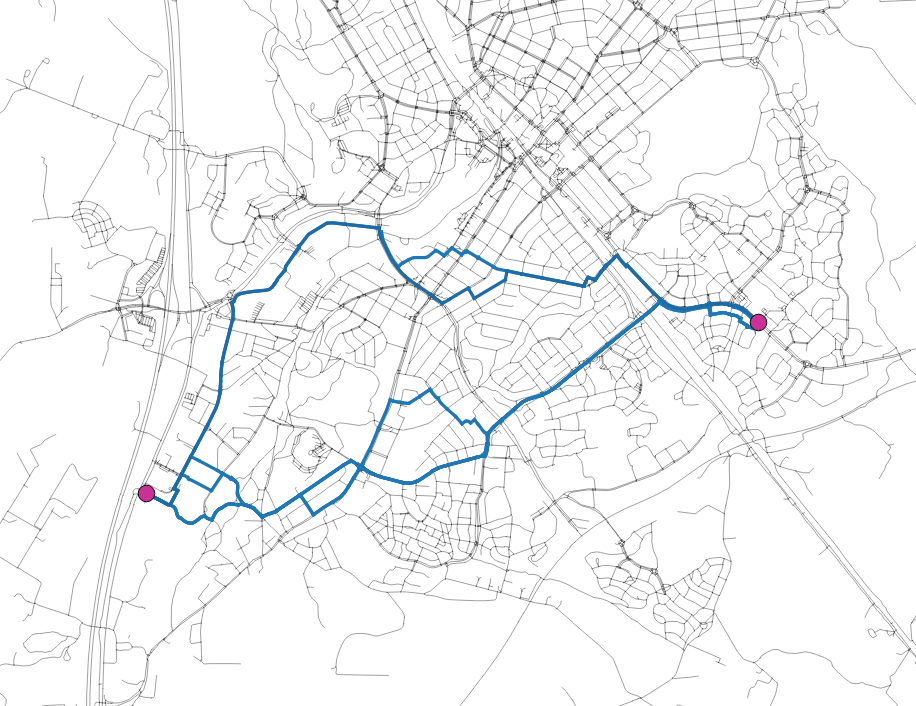
\includegraphics[width=12cm]{img/c01-transp-model/paths.png}
  \label{img.paths}
  \caption{Possible paths between one pair of zone (multipath)}
\end{figure}
% TM - Data Structure
%%%%%%%%%%%%%%%%%%%%%%%%%%%%%%%%%%%%%%%%%%%%%

%%%%%%%%%%%%%%%%%%%%%%%%%%%%%%%%%%%%%%%%%%%%%%%%%%%%%%%%%%%%%%%%%%%%%%%%%

% EN
%\section{Implementation}

% FR
\section{Implémentation}

% EN
% In upcoming section following expressions will be used:

% \begin{tabular}{ll}
%   $n$ & number of nodes\\
%   $m$ & number of edges \\
%   $z$ & number of zones\\
%   $N$ & number of path computed for one pair of zone
% \end{tabular}

% Transportation modelling described in previous section was implemented in Python programming language using NumPy library.

% FR
Dans cette section, les expressions suivantes vont être utilisées :

\begin{tabular}{ll}
  $n$ & nombre de noeuds\\
  $m$ & nombre de bords \\
  $z$ & nombre de zone\\
  $N$ & nombre de chemin calculé pour une paire de zone
\end{tabular}

La modélisation de transport décrits dans la section précédente a été mise en œuvre dans le langage de programmation Python en utilisant la bibliothèque NumPy.

%%%%%%%%%%%%%%%%%%%%%%%%%%%%%%%%%%%%%%%%%%%%%%%%%%%%%%%%%%%%%%%%%%%%%%%%%

% EN
%\subsection{Static shortest path search}

% FR
\subsection{Recherche du plus court chemin statique}

% EN
% For determined $C$ we use Dijkstra's algorithm (complexity $O(m +n log(n) )$). So final complexity is 
% $$O(z (m + n log(n)))$$
% For traffic count we used also Dijkstra's algorithm. Final complexity for traffic count is 
% $$O(N z (m + n log(n)))$$
% For Dijkstra's algorithm we used Python library iGraph. iGraph is written in C programming language so it is quite fast. For example one Dijkstra running 30 ms ($n = 8000$ $m = 18000$).

% FR
Pour déterminer $C$ nous utilisons l'algorithme de Dijkstra's (de complexité $O(m +n log(n) )$). De fait, la complexité finale est de
$$O(z (m + n log(n)))$$
For traffic count we used also Dijkstra's algorithm. Final complexity for traffic count is 
$$O(N z (m + n log(n)))$$
For Dijkstra's algorithm we used Python library iGraph. iGraph is written in C programming language so it is quite fast. For example one Dijkstra running 30 ms ($n = 8000$ $m = 18000$).

%%%%%%%%%%%%%%%%%%%%%%%%%%%%%%%%%%%%%%%%%%%%%%%%%%%%%%%%%%%%%%%%%%%%%%%%%
\subsection{Data store}
All data for transportation modelling are stored in relation database PostgreSQL with extension PostGIS. PostGIS is spatial extension. Using it you can manipulate with line, point, polygon, raster.

In database there are 6 main table:

\begin{tabular}{|l|l|}
\hline
Table name & \\
\hline
\hline
\textbf{roads} & road links (edges)\\
\textbf{nodes} & nodes (vertexes)\\
\textbf{zones} & list of zones\\ 
\textbf{traffic} & \\
\textbf{general\_area\_information} & contains interested area geometry\\
\textbf{od\_pair} & Database implementation for $T$ matrix\\
\hline
\end{tabular}

In Fig \ref{img.schema} there are all table in database model and relationships between them (arrow is FOREIGN KEY).

\begin{figure}
\centering
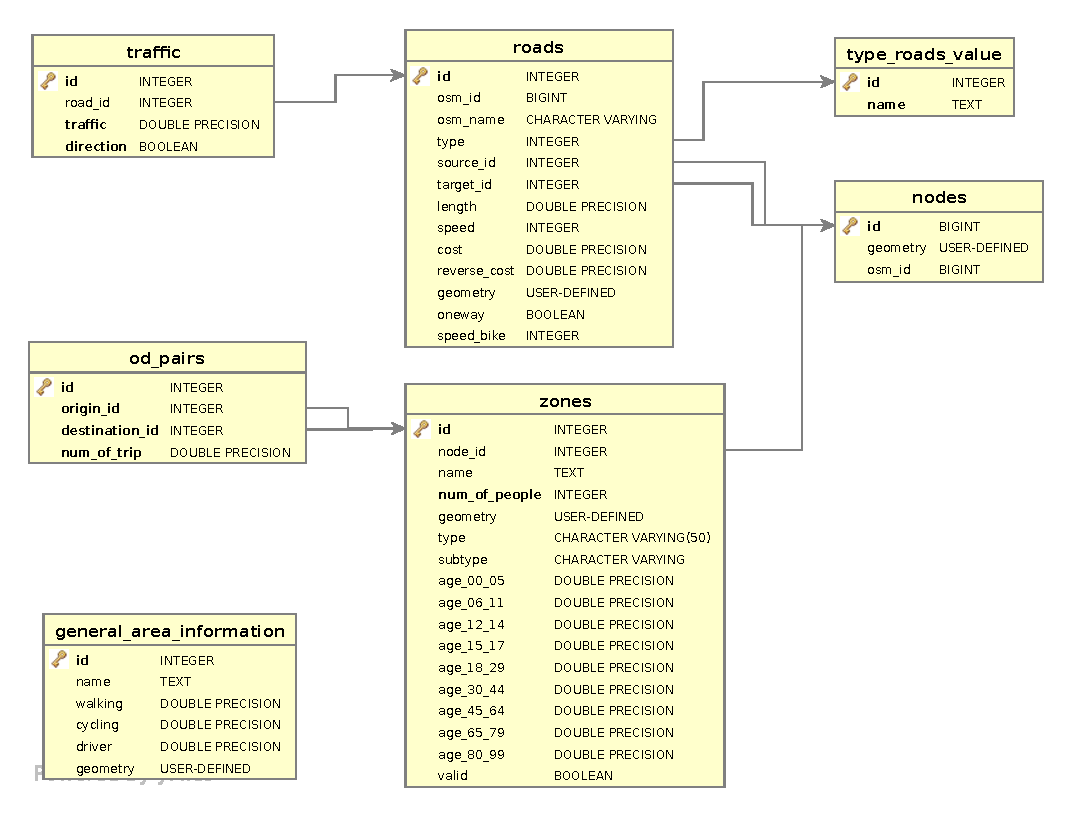
\includegraphics[width=15cm]{img/c01-transp-model/db.eps}
\caption{Database model}
\label{img.schema}
\end{figure}

More details about DB you can find in project documentation on GitHub.

%%%%%%%%%%%%%%%%%%%%%%%%%%%%%%%%%%%%%%%%%%%%%%%%%%%%%%%%%%%%%%%%%%%%%%%%%
\subsection{Future work}
This method of transportation modelling is very hard ($O(N z (m + n log(n)))$), so it is suitable compute this problem in some parallel environment (shared (Threads) or distributed memory (MapReduce or MPI)).


% TM - Practice
%%%%%%%%%%%%%%%%%%%%%%%%%%%%%%%%%%%%%%%%%%%%%

%%%%%%%%%%%%%%%%%%%%%%%%%%%%%%%%%%%%%%%%%%%%%%%%%%%%%%%%%%%%%%%%%%%%%%%%%

\section{Practice - implementation as REST Service}
The project have 3 main goal tool for transportation modelling and web application for it. So we had to make REST service. This service is based on python micro-framework Flask. In Fig. \ref{img.b} you can see all backend environment.

\begin{figure}
\centering
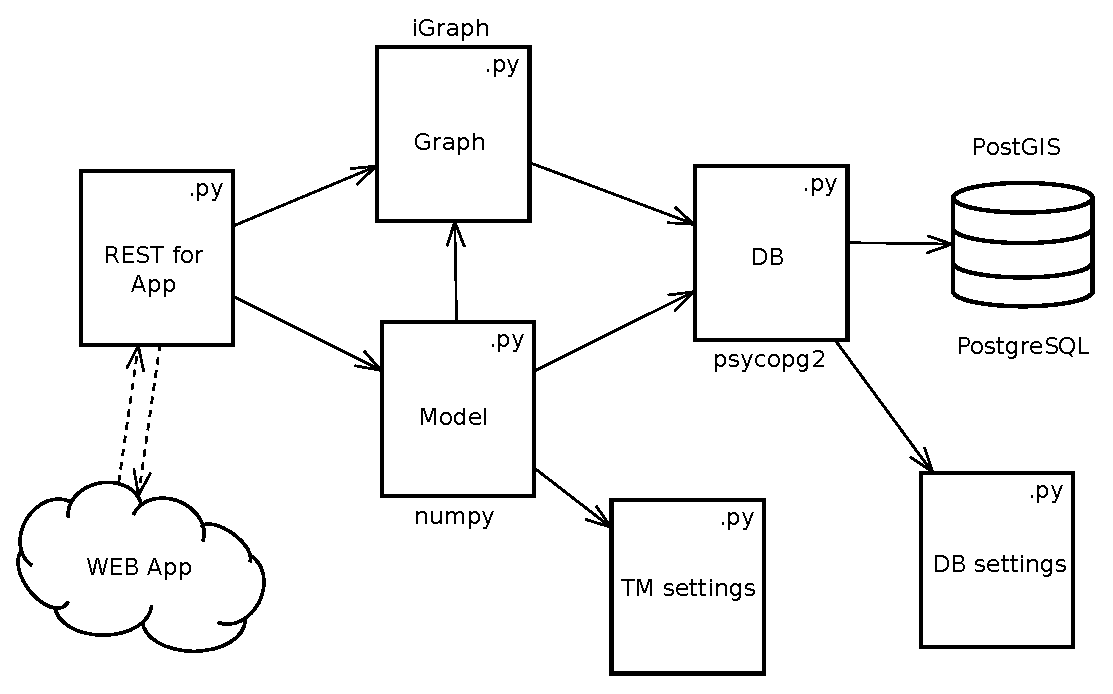
\includegraphics[width=15cm]{img/c01-transp-model/backend.eps}
\caption{Backend (REST)}
\label{img.b}
\end{figure}

Recompute traffic take a lot of time, so REST must be asynchronous. In our approach we made two service. First service start compute and second return progress.

Example:
\begin{verbatim}
/api/compute_traffic

{"status": "ok", "result": "calculation began"}

/api/compute_traffic_progress

{"status": "ok", "result": {"progress": 34, "isrun": true}}
\end{verbatim}

\chapter{Web content}
% Application - Prototypes
%%%%%%%%%%%%%%%%%%%%%%%%%%%%%%%%%%%%%%%%%%%%%

% FR
Avant d'entamer le développement de l'application, il est nécessaire de faire un état du besoin et des attentes. Ainsi, en structurant notre interface il sera plus facile de procéder à son développement graphique, d'anticiper les classes et fonctions nécessaires aux traitements. Dans un premier temps, nous allons structurer nos interfaces afin d'être au plus proche des attentes utilisateurs, puis nous détaillerons les outils à notre disposition et comment ils fonctionnent, et enfin nous procèderons au dévelopement de l'application cliente.

% EN
%Before starting the development of the application, it is necessary to make a statement of needs and expectations. Thus, by structuring our interface will make it easier to conduct its graphic development, anticipate the classes and functions necessary for treatment. Initially, we will structure our interfaces in order to be closer to the users expectations, then we will detail the tools available and how they work, and then we will proceed to the developement of the client application.

%%%%%%%%%%%%%%%%%%%%%%%%%%%%%%%%%%%%%%%%%%%%%%%%%%%%%%%%%%%%%%%%%%%%%%%%%
% FR
\section{Prototypes}

% EN
%\section{Prototypes}

% FR
Dans ce paragraphe nous allons détailler chacune des interfaces qui seront implémentées dans l'application. L'application sera construite sous deux angles différents :
\begin{description}
  \item[La partie cartographique :] \hfill \\ contenant une carte de base et dont les outils se superposent à cette dernière
  \item[La partie site web :] \hfill \\ contenant des outils indépendants de la carte
\end{description}

% EN
% In this section we will detail each of the interfaces that will be implemented in the application. The application will be built in two different ways:
% \begin{description}
%   \item[Map content :] \hfill \\ containing a basemap and whose tools are over the map
%   \item[Website content :] \hfill \\ containing independent map tools
% \end{description}

% FR
\subsection{Partie cartographique}

% EN
%\subsection{Map content}

% FR
Le contenu cartographique détermine la base de notre application. En effet, cette dernière est constituée de trois éléments important : le fond de carte, la table des matières et les boutons d'interraction avec la carte.

% EN
%The map content determines the basis of our application. Indeed, the latter consists of three major components: the base map, table of contents and the interraction with map buttons.



% BASEMAP
% ----------------------------------------------

\begin{figure}[ht]
  \centering
  \begin{subfigure}[b]{0.6\textwidth}
    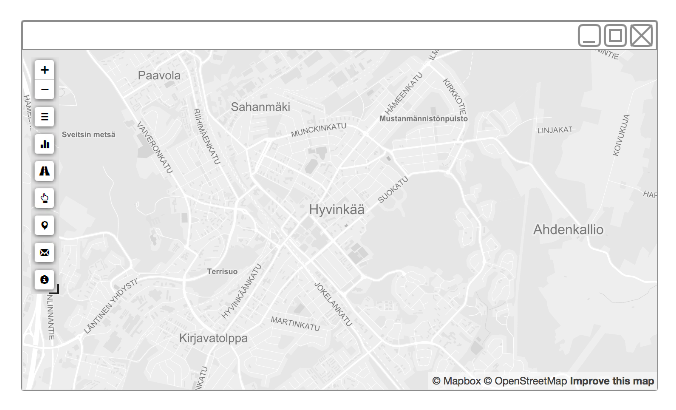
\includegraphics[width=\textwidth]
      {img/c02-application/png/web-basemap.png}
    \caption{Web}
  \end{subfigure}
  ~
  \begin{subfigure}[b]{0.2\textwidth}
    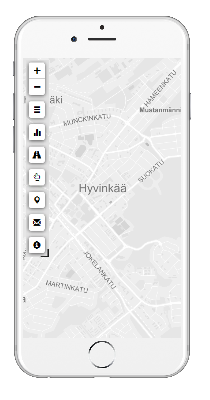
\includegraphics[width=\textwidth]
      {img/c02-application/png/mobile-basemap.png}
    \caption{Mobile}
  \end{subfigure}
  \caption{Application: Basemap}
\end{figure}

% EN
%The base map allows you to locate geographically in a recognizable environment. It shall be set up raster image on which we will be able to overlay vector data from the server. For our application we will build on the maps tiles proposed by MapBox.



% FR 
Le fond de carte permet de se repérer géographiquement dans un environnement reconnaissable. Il est consitué d'image raster sur lesquelles on va pouvoir superposer les données vectorielles issues du serveur. Pour notre application nous allons nous appuyer sur les fonds de carte proposé par MapBox.


% TOC
% ----------------------------------------------

\begin{figure}[ht]
  \centering
  \begin{subfigure}[b]{0.6\textwidth}
    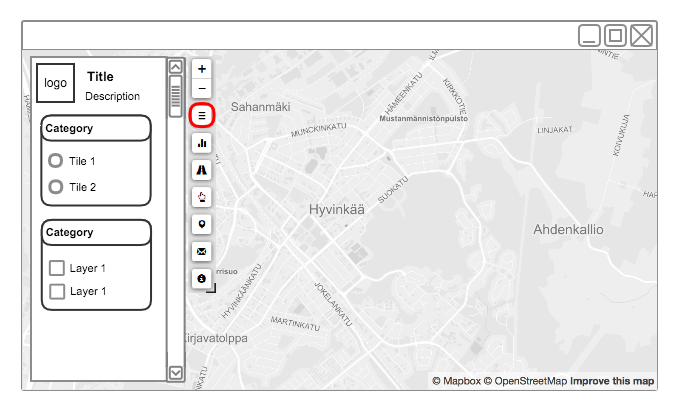
\includegraphics[width=\textwidth]
      {img/c02-application/png/web-basemap-toc.png}
    \caption{Web}
  \end{subfigure}
  ~
  \begin{subfigure}[b]{0.2\textwidth}
    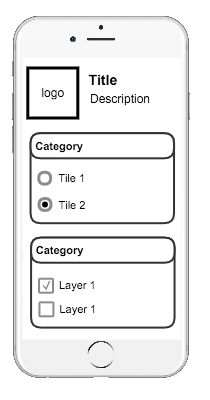
\includegraphics[width=\textwidth]
      {img/c02-application/png/mobile-basemap-toc.png}
    \caption{Mobile}
  \end{subfigure}
  \caption{Application: Table Of Content}
\end{figure}

% FR
La table des matières, ou \textit{Table of Content} (en anglais, abrégé TOC), permet de lister les élements de la carte et de pouvoir interagir avec eux. Elle contiendra les différentes couches, ou \textit{Layer} en anglais, constitutives de l'application. Des checkbox ou bouton radio devraient s'y trouver pour afficher ou masquer des éléments.

Les boutons d'interractions sont de trois types : le déclenchement d'action par dessus la carte (popup), le déclenchement d'action avec une interraction sur la carte, ou l'ouverture d'une page spécifique du minisite.

% EN
%The table of contents (abbreviated TOC) can list the elements of the map and interact with them. It will contain the different layers component of the application. The checkbox or radio button should be there to show or hide items.

%The interractions buttons are of three types: the onset of action over the map (popup), the onset of action with interraction on the map (marker), or open a specific page of the mini-website.

% SEARCH POINTER
% ----------------------------------------------

% FR
Parmis les boutons d'action sur la carte, un outils indispensable est la recherche d'itinéraire. Ce bouton permet d'activer la dépose de marker à la main directement sur la carte pour placer deux points qui serviront de départ et d'arrivée. Après avoir déposé les markers, un itinéraire le plus court est calculé et affiché sur la carte.

% EN
%Among the action buttons on the map, an indispensable tool is the route search. This button turns the marker removal by hand directly on the map to place two points that serve as departure and arrival. After dropping the markers, the shortest route is calculated and displayed on the map.

\begin{figure}[ht]
  \centering
  \begin{subfigure}[b]{0.6\textwidth}
    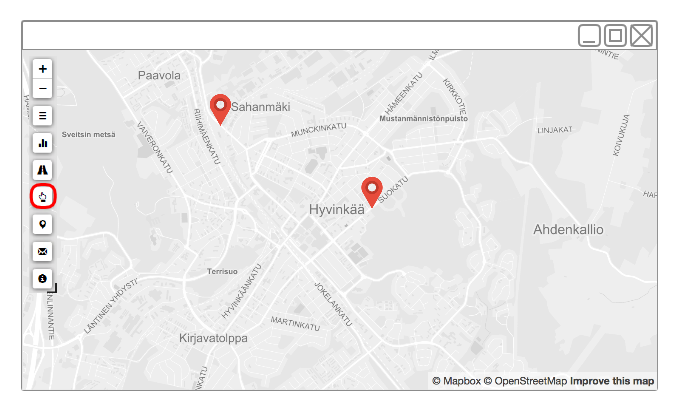
\includegraphics[width=\textwidth]
      {img/c02-application/png/web-basemap-search.png}
    \caption{Web}
  \end{subfigure}
  ~
  \begin{subfigure}[b]{0.2\textwidth}
    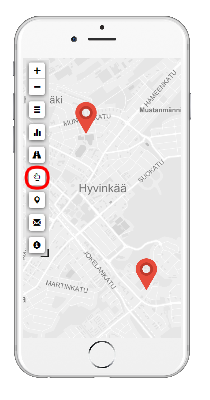
\includegraphics[width=\textwidth]
      {img/c02-application/png/mobile-basemap-search.png}
    \caption{Mobile}
  \end{subfigure}
  \caption{Application: SearchPointer}
\end{figure}

% FOCUS
% ----------------------------------------------

% FR
Un autre des outils nécessaires au bon fonctionnement de l'application est un bouton permettant de se géolocaliser. Ce bouton ouvre une popup par dessus la carte permettant de choisir de se localiser par mot clef ou bien par coordonnées (latitude et longitude).

% EN
%Another of the tools necessary for the application is a button to geotag. This button opens a popup over the map to choose to locate by keyword or by coordinates (latitude and longitude).

\begin{figure}[ht]
  \centering
  \begin{subfigure}[b]{0.6\textwidth}
    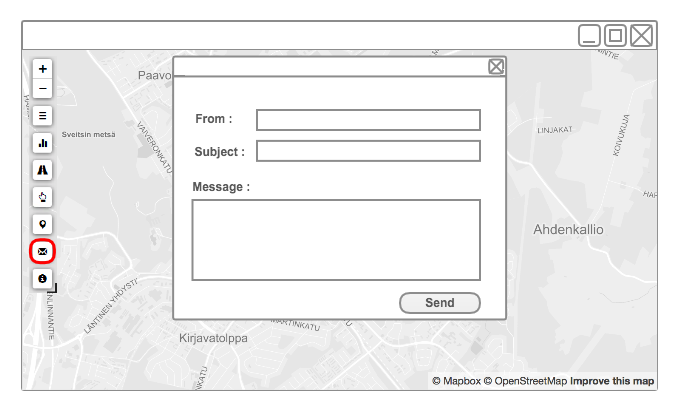
\includegraphics[width=\textwidth]
      {img/c02-application/png/web-basemap-focus.png}
    \caption{Web}
  \end{subfigure}
  ~
  \begin{subfigure}[b]{0.2\textwidth}
    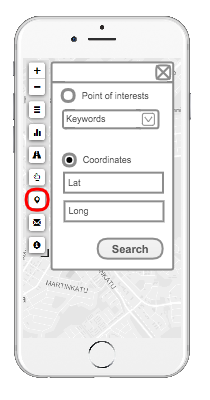
\includegraphics[width=\textwidth]
      {img/c02-application/png/mobile-basemap-focus.png}
    \caption{Mobile}
  \end{subfigure}
  \caption{Application: Focus}
\end{figure}

% CONTACT
% ----------------------------------------------

% FR
Les deux derniers boutons qui doivent être ajoutés ne sont pas nécessaires pour l'application mais simplement utiles et informatifs. Il s'agit des boutons de contact et d'information à propos de l'application. Ces deux boutons ouvre une popup par dessus la carte. Le bouton de contact propose un formulaire permettant de directement envoyer un message aux développeurs de l'application. Quant au bouton d'information, c'est une simple surcouche permettant d'afficher des informations sur les développeurs et les sources de l'application.

% EN
%The last two buttons that need to be added are not necessary for the application but merely useful and informative. These are contact buttons and information about the application. These two buttons open a popup over the map. The contact button provides a form to send a message directly to the developers of the application. As for the information button is a simple overlay that displays information about the developers and the sources of the application.

\begin{figure}[ht]
  \centering
  \begin{subfigure}[b]{0.6\textwidth}
    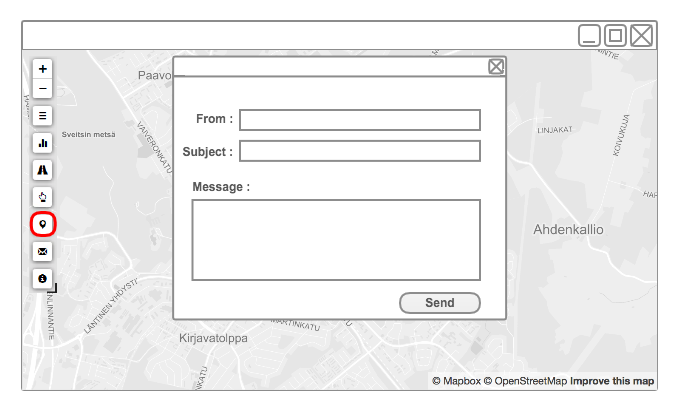
\includegraphics[width=\textwidth]
      {img/c02-application/png/web-basemap-contact.png}
    \caption{Web}
  \end{subfigure}
  ~
  \begin{subfigure}[b]{0.2\textwidth}
    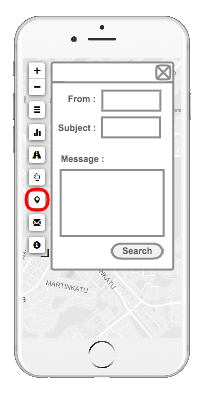
\includegraphics[width=\textwidth]
      {img/c02-application/png/mobile-basemap-contact.png}
    \caption{Mobile}
  \end{subfigure}
  \caption{Application: Contact}
\end{figure}

%%%%%%%%%%%%%%%%%%%%%%%%%%%%%%%%%%%%%%%%%%%%%%%%%%%%%%%%%%%%%%%%%%%%%%%%%

% FR
\subsection{Partie site web}

% EN
%\subsection{Website content}

% FR
Les derniers boutons qui n'ont pas été détaillés dans la partie précédent sont les liens directs vers le mini-site internet. En effet, Il est plus aisé d'aller directement sur le contenu souhaité depuis la carte plutôt que de naviguer sur le site. Parmis les boutons non explicités, on retrouve un bouton d'accès aux statistiques et aux horaires de trains.

% EN
%The last buttons that were not detailed in the previous section are direct links to the Internet website content. Indeed, it is easier to go directly to the desired content from the map rather than browse in the site. Among the non-explicit buttons, we have a button access to statistics and trains timetables.

% STATS
% ----------------------------------------------

% FR
Le site web est composé d'une petite barre de navigation en haut de la page et d'un contenu central. Un lien dans la barre de navigation nous permet de revenir sur la carte. Le contenu central de la page change selon la page désirée. 

Le contenu central de la partie statistique est une liste de schéma et d'un schéma global qui s'actualise selon l'objet sélectionné sur la liste.

% EN
%The website consists of a small top navigation bar and a central content. A link in the navigation bar allows us to go back on the map. The central content of the page changes depending on the desired chart.

%The central content of the statistical part is a charts list and an overall chart that is updated as the selected object on the list.

\begin{figure}[ht]
  \centering
  \begin{subfigure}[b]{0.6\textwidth}
    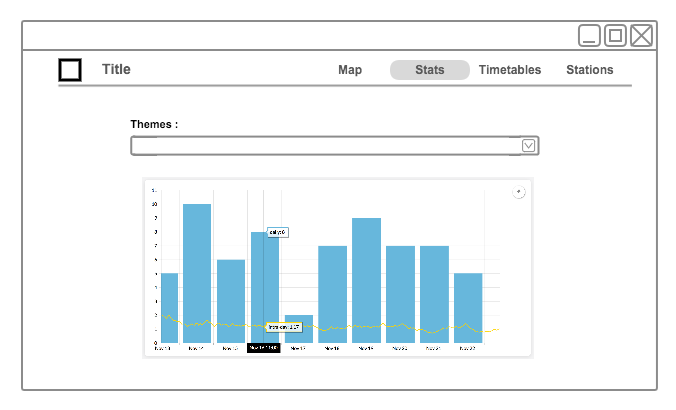
\includegraphics[width=\textwidth]
      {img/c02-application/png/web-website-stats.png}
    \caption{Web}
  \end{subfigure}
  ~
  \begin{subfigure}[b]{0.2\textwidth}
    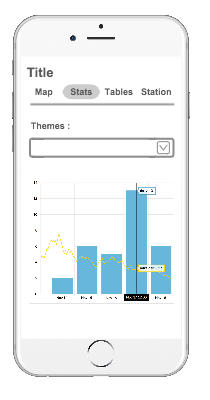
\includegraphics[width=\textwidth]
      {img/c02-application/png/mobile-website-stats.png}
    \caption{Mobile}
  \end{subfigure}
  \caption{Application: Statistics}
\end{figure}

% TIMETABLES
% ----------------------------------------------

% FR
En ce qui concerne les horaires de train, il s'agit d'une interface permettant de récupérer les trains qui intéressent l'utilisateur. L'utilisateur à alors le choix de lister tous les départs de train d'une ville, toutes les arrivées d'une ville ou bien de déterminer l'itinéraire entre deux villes. Une fois le choix fait, l'utilisateur renseigne les villes désirées dans les zones concernées. L'application récupère alors les données et les affiches à l'utilisateur sous forme de liste à ouvrir.

% EN
%Regarding train schedules, it is an interface to retrieve the trains that interest the user. The user then has the choice of listing all train departures of a city, all arrivals to a city or to determine the route between two cities. The choice made, the user fills in the desired towns in the affected areas. The application then retrieves the data and signs the user in a list to open.

\begin{figure}[ht]
  \centering
  \begin{subfigure}[b]{0.6\textwidth}
    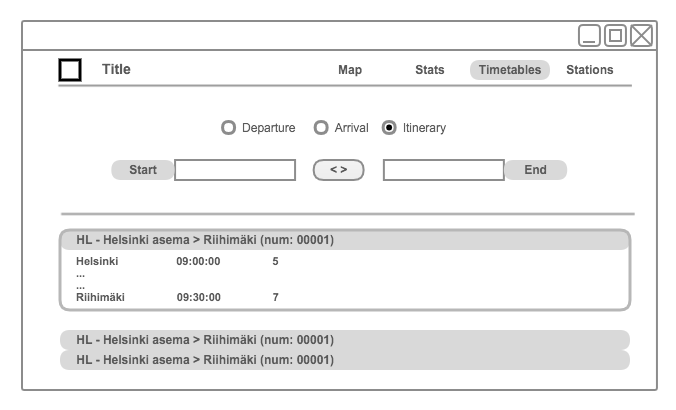
\includegraphics[width=\textwidth]
      {img/c02-application/png/web-website-timetables.png}
    \caption{Web}
  \end{subfigure}
  ~
  \begin{subfigure}[b]{0.2\textwidth}
    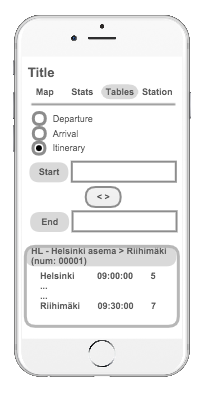
\includegraphics[width=\textwidth]
      {img/c02-application/png/mobile-website-timetables.png}
    \caption{Mobile}
  \end{subfigure}
  \caption{Application: Timetables}
\end{figure}

% Application - Code
%%%%%%%%%%%%%%%%%%%%%%%%%%%%%%%%%%%%%%%%%%%%%

% FR
\section{Développement de l'application}

% EN
%\section{Application's Development}

% FR
Pour obtenir un code efficace, maintenable et évolutif, il est nécessaire de devoir penser à la fléxibilité de celui-ci. En effet, plus il est possible d'ajouter des fonctionnalité, des outils et de personnaliser son environnement, plus l'outil est polyvalent.

% EN
%For an efficient, scalable and maintainable code, it is necessary to have to think about the flexibility of it. Indeed, it is possible to add functionality, tools and customize its environment, the tool is more versatile.

%%%%%%%%%%%%%%%%%%%%%%%%%%%%%%%%%%%%%%%%%%%%%%%%%%%%%%%%%%%%%%%%%%%%%%%%%%%%%%

% FR
\subsection{Environnement}

% EN
%\subsection{Environment}

% FR
Avant d'entamer le coeur du développement, il est nécessaire de rappeler l'environnement dans lequel l'application est développée. 

L'application doit être utilisable sur un environnement web, sur bureau et sur mobile. De fait, l'application peut être consultable depuis un navigateur web. Il est également intéressant de penser dès maintenant à la protabilité vers une application mobile (Android, iOS, Windows Phone, FirefoxOS). Un code modulable est intéressant, mais encore plus s'il peut être adapté selon les plateformes désirées.

Coté serveur, nous disposerons de toutes les informations cartographiques nécessaires. Pour celà, il faut pouvoir construire un serveur ouvert sur internet et pouvant répondre aux requêtes web venant de l'application.

Les technologies choisies sont donc :

\begin{description}

  \item[Serveur] \hfill 
    \begin{itemize}
      \item Apache2 : Le logiciel libre Apache HTTP Server (Apache) est un serveur HTTP créé et maintenu au sein de la fondation Apache. Il servira de serveur Web.
      \item Tomcat7 : Apache Tomcat est un conteneur web libre de servlets et JSP Java EE. Il servira à faire tourner les sources GéoServer.
      \item GéoServer : GéoServer est un serveur informatique open source et libre écrit en Java qui permet aux utilisateurs de partager et modifier des données géographiques. Il contiendra nos informations cartographiques.
      \item REST Services : Les services web de type Representational state transfer (REST) exposent entièrement des fonctionnalités comme un ensemble de ressources (URI) identifiables et accessibles par la syntaxe et la sémantique du protocole HTTP. Ce type de service est exécutée par un script Python en Deamon.
    \end{itemize}

  \item[Application] \hfill 
    \begin{itemize}
      \item HTML : L’Hypertext Markup Language, généralement abrégé HTML, est le format de données conçu pour représenter les pages web. 
      \item CSS : Les feuilles de style en cascade est un langage informatique qui décrit la présentation des documents HTML et XML. Ce langage permettra de donner un style à notre application.
      \item Javascript : JavaScript est un langage de programmation de scripts principalement employé dans les pages web interactives mais aussi pour les serveurs. Ce langage nous permettra de faire les interractions entre notre contenu HTML et nos données SIG contenu sur le serveur. Il permettra de gérer les interractions.
    \end{itemize}

  \item[Frameworks et Utilitaires] \hfill \\
    En programmation informatique, un framework ou structure logicielle est un ensemble cohérent de composants logiciels structurels, qui sert à créer les fondations ainsi que les grandes lignes de tout ou d’une partie d'un logiciel. Nous allons nous appuyer sur différents frameworks et utilitaires pour notre application :
    \begin{itemize}
      \item Bootstrap : Twitter Bootstrap est une collection d'outils HTML, CSS et JavaScript utiles à la création de sites et d'applications web.
      \item Leaflet : Leaflet est une bibliothèque logicielle libre en JavaScript de cartographie interactive.
      \item JQuery : jQuery est une bibliothèque JavaScript libre et multi-plateforme créée pour faciliter l'écriture de scripts côté client dans le code HTML des pages web.
      \item AmCharts : amCharts est une bibliothèque Javascript de graphiques qui répond à tous les besoins de visualisation de données.
      \item Cordova : Apache Cordova est un framework de développement mobile open-source. Il permet d'exploiter les technologies Web courantes telles que HTML5, CSS3 et JavaScript pour développer des applications multi-plateformes, évitant ainsi l'utilisation des langages natifs propres aux différentes plates-formes mobiles.
    \end{itemize}

\end{description}


% EN

% Before beginning the core's development, it is necessary to remind the environment in which the application is developed.

% The application must be used on a web environment, desktop and mobile. In fact, the application can be viewed from a web browser. It is also interesting to think now in protabilité to a mobile application (Android, iOS, Windows Phone, FirefoxOS). A modular code is interesting, but even more if it can be adapted as desired platforms.

% Server side, we will have all the map information needed. For that, we need to build an server open on the internet and can respond to web requests from the application.

% The selected technologies are:

% \begin{description}

%   \item[Server] \hfill 
%     \begin{itemize}
%       \item Apache2 : Free software Apache HTTP Server (Apache) is an HTTP server created and maintained within the Apache Foundation. It will serve as Web server.
%       \item Tomcat7 : Apache Tomcat is a web container free of servlets and JSP Java EE. It will be used to execute the GeoServer's sources.
%       \item GeoServer : GeoServer is an open-source server written in Java - allows users to share, process and edit geospatial data.
%       \item REST Services : The REST web services (Representational state transfer) fully expose functionality as a set of resources (URI) identifiable and accessible by the syntax and semantics of HTTP. This type of service is performed by a Python script Deamon.
%     \end{itemize}

%   \item[Application] \hfill 
%     \begin{itemize}
%       \item HTML : HyperText Markup Language, commonly referred to as HTML, is the standard markup language used to create web pages.
%       \item CSS : Cascading Style Sheets, CSS, is a style sheet language used for describing the presentation of a document written in a markup language. This language will give style to our application.
%       \item Javascript : JavaScript is a high-level, dynamic, untyped, and interpreted programming language. This language will allow us to interactions between our HTML content and our GIS data content on the server. It will manage interractions.
%     \end{itemize}

%   \item[Frameworks and Tools] \hfill \\
%     A software framework is an abstraction in which software providing generic functionality can be selectively changed by additional user-written code, thus providing application-specific software. A software framework is a universal, reusable software environment that provides particular functionality as part of a larger software platform to facilitate development of software applications, products and solutions. We will use different frameworks and utilities for our application:
%     \begin{itemize}
%       \item Bootstrap : Bootstrap is a free and open-source collection of tools in HTML, CSS and Javascript for creating websites and web applications.
%       \item Leaflet : Leaflet is a widely used open source JavaScript library used to build web mapping applications.
%       \item JQuery : jQuery is a cross-platform JavaScript library designed to simplify the client-side scripting of HTML.
%       \item AmCharts : JavaScript / HTML5 charts and maps library for web sites and web applications. Fast and responsive.
%       \item Cordova : Apache Cordova is an open-source mobile development framework. It allows you to use standard web technologies such as HTML5, CSS3, and JavaScript for cross-platform development, avoiding each mobile platforms' native development language.
%     \end{itemize}

% \end{description}

%%%%%%%%%%%%%%%%%%%%%%%%%%%%%%%%%%%%%%%%%%%%%%%%%%%%%%%%%%%%%%%%%%%%%%%%%%%%%%

% FR
\subsection{Architecture de l'application}

% EN
%\subsection{Application architecture}

% FR
Le serveur ne nécessitant pas de structure particulière (un simple script REST excuté en Deamon et trois serveurs auto-gérés) nous allons détailler la structure de l'application.

L'application s'articule sur une pseudo-architecture MVC (model, view, controller). Une seule page HTML est nécessaire pour obtenir la cartographie de base, des scripts JavaScript vont servir de controller pour charger les données et des pages HTML contiendront les informations des Popup sous forme de views.

De fait, nous pouvons imaginer la structure de l'application de la manière suivante : 
\noindent\fbox{\parbox{\linewidth\fboxrule\fboxsep}{
  \dirtree{%
    .1 /sources.
    .2 /config.
    .3 \textit{(fichier de configuration json)}.
    .2 /css.
    .3 \textit{(style de l'application)}.
    .2 /img.
    .3 \textit{(les sources d'imagerie)}.
    .2 /js.
    .3 \textit{(fichier de chargement et d'évènement javascript)}.
    .2 /lib.
    .3 \textit{(sources des frameworks et outils)}.
    .2 /views.
    .3 \textit{(sources HTML des différents affichages)}.
    .2 index.html.
  }
}}

% EN
% The server does not require a special structure (a simple REST script executes in Deamon and three self-managed servers) we will detail the application's structure.

% The application is based on a pseudo-architecture MVC (model, view, controller). A single HTML page is required for the base mapping, JavaScript will serve as controller to load the data and HTML pages contain information Popup in the form of views.

% In fact, we can imagine the structure of the application like this: \\
% \noindent\fbox{\parbox{\linewidth\fboxrule\fboxsep}{
%   \dirtree{%
%     .1 /sources.
%     .2 /config.
%     .3 \textit{(json configuration files)}.
%     .2 /css.
%     .3 \textit{(app's style files)}.
%     .2 /img.
%     .3 \textit{(pictures ressources)}.
%     .2 /js.
%     .3 \textit{(javascript class, loader and event files)}.
%     .2 /lib.
%     .3 \textit{(frameworks and tools sources)}.
%     .2 /views.
%     .3 \textit{(HTML sources for differents views)}.
%     .2 index.html.
%   }
% }}

%%%%%%%%%%%%%%%%%%%%%%%%%%%%%%%%%%%%%%%%%%%%%%%%%%%%%%%%%%%%%%%%%%%%%%%%%%%%%%

% FR
\subsubsection{Configuration JSON}

% EN
%\subsubsection{JSON Configuration}

% FR
Dans le paragraphe précédent et sur schéma proposé, il est question d'un dossier de configuration JSON. En effet, pour éviter la redondance des fonctions et pour une meilleure fleibilité, il est plus facile d'utiliser un fichier de configuration JSON couplé à une classe JavaScript contenant des Getters. Nous utiliserons ainsi, quatre fichiers de configurations :

\begin{itemize}
  \item configMap : Ce fichier contient les configurations par défaut de la carte à charger (zoom, centre, position de la TOC)
  \item configContent : Ce fichier contient les noms des balises HTML qui recevront les informations des Popup, mais également les liens vers les views des popup, leur nom et leur icon.
  \item configServer : Ce fichier contient les accès au serveur. Notamment les configurations pour le GéoServer et pour l'API REST
  \item configLayerStyle : Ce fichier est l'un des plus important, il contient les styles graphiques à appliquer pour chaque couches à superposer sur la carte. Notamment, le nom à afficher à l'utilisateur, les niveaux de zoom minimum et maximum, les couleurs et les styles visuels des couches.
\end{itemize}


% EN
% In the previous paragraph and the proposed scheme, there is talk of a JSON configuration file. Indeed, to avoid duplication of functions and greater flexibility, it is easier to use a JSON configuration file coupled with a JavaScript class containing Getters. We will use four configuration files:

% \begin{itemize}
%   \item configMap : This file contains the default configurations of the map to load (zoom, center, TOC position)
%   \item configContent : This file contains the names of HTML tags that will receive information Popup but also links to popup views, their name and icon.
%   \item configServer : This file contains the server access. Including configurations for GeoServer and the REST API
%   \item configLayerStyle : This file is one of the most important, it contains graphic styles to be applied to each layer superimposed on the map. In particular, the name to be displayed to the user, the minimum and maximum zoom levels, colors and visual styles of the layers.
% \end{itemize}

%%%%%%%%%%%%%%%%%%%%%%%%%%%%%%%%%%%%%%%%%%%%%%%%%%%%%%%%%%%%%%%%%%%%%%%%%%%%%%

% FR
\subsubsection{Classes}

% EN
%\subsubsection{Classes}

% FR
Chacun des fichiers JSON de configuration possède au moins une classe Javascript dans le répertoire ``/js'' qui lui est associé. En effet, comme expliqué dans le paragraphe précédent, il est plus facile d'utiliser des objets et des outils comme des Getters et Setters pour accéder à un fichier de configuration JSON. De fait, nous avons les classes suivantes : 

\begin{itemize}
  \item classMapProperties : Permet de récupérer toutes les informations relatives à la carte contenu dans le fichier configMap.json
  \item classGeoServerProperties : Permet de récupérer toutes les informations relatives au GeoServer contenu dans le fichier configServer.json
  \item classRestProperties : Permet de récupérer toutes les informations relatives à l'API REST contenu dans le fichier configServer.json
  \item classContentProperties : Permet de récupérer toutes les informations relatives aux contenus des Popup à afficher au dessus de la carte dans le fichir configContent.json
  \item classLayerStyleProperties : Permet de récupérer toutes les informations relatives aux layers contenus dans le fichier configLayerStyle.json
  \item classLayerProperties : Cette classe ne dépend pas d'un fichier de configuration, elle permet de structurer un Layer avec des attributs permettant des interractions entre la carte et la table des matières (TOC). Un objet issu de cette classe possèdera alors un nom, un alias, une position, un type de couche, une URL vers la couche sur le GeoServer ainsi que l'objet cartographique à afficher.
\end{itemize}

% EN

% Each of the configuration files JSON Javascript has at least one class in the `` /js '' associated with it. Indeed, as explained in the previous paragraph, it is easier to use objects and tools Getters and Setters like to access a JSON configuration file. In fact, we have the following classes:

% \begin{figure}[ht]
%   \centering
%   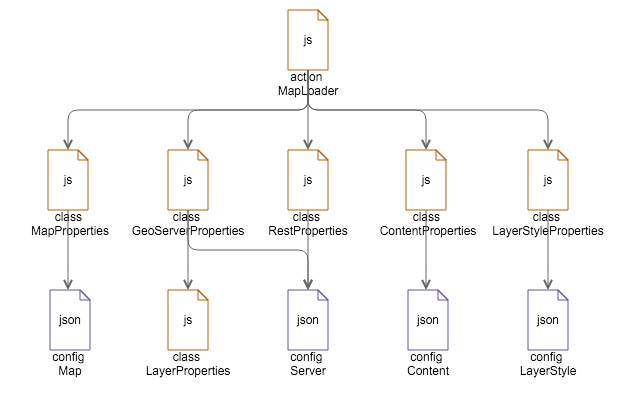
\includegraphics[width=12cm]{img/c02-application/png/app-class-loading.png}
%   \caption{Loading JSON and Classes}
% \end{figure}

% \begin {itemize}
%   \item classMapProperties: Retrieves all information about the map contained in the file configMap.json
%   \item classGeoServerProperties: Retrieves all information relating to GeoServer contained in the file configServer.json
%   \item classRestProperties: Retrieves all information related to the REST API contained in the file configServer.json
%   \item classContentProperties: Retrieves all information about Popup content to be displayed above the map in the file configContent.json
%   \item classLayerStyleProperties: Retrieves all information about layers contained in the file configLayerStyle.json
%   \item classLayerProperties: This class does not depend on a configuration file, it allows to structure a Layer with attributes allowing interractions between the map and the table of contents (TOC). An object from this class will then have a name, an alias, a position, a type layer, a URL to the layer on the GeoServer and map item to display.
% \end {itemize}


%%%%%%%%%%%%%%%%%%%%%%%%%%%%%%%%%%%%%%%%%%%%%%%%%%%%%%%%%%%%%%%%%%%%%%%%%%%%%%

% FR
\subsubsection{Evènements}

% EN
%\subsubsection{Events}

% FR
Le coeur de l'application est concentrée dans des fichiers Javascript préfixés par ``action...''. Chacun de ces fichiers, triés par thème, permet de générer le contenu de la carte. Dans nos sources, les fichiers sont chargés dans l'ordre suivant afin d'obtenir toutes les fonctions nécessaires avant de charger la totalité de la carte : 

\begin {itemize}
  \item Les fichiers Javascript des différents Frameworks (jQuery, Bootstrap, Extensions de Bootstrap, Leaflet, Extensions de Leaflet).
  \item Les fichiers de classes associés aux configurations JSON du paragraphe précédent.
  \item actionPopup : Ce fichier contient les fonctions relatives aux popup renseignées dans le fichier de configuration JSON des Popup. En effet, chaque popup dispose de ses fonctions, de ses interractions avec la carte et de ses spécificités. Parmis ces fonctions, nous chargeons également le contenu HTML des popup qui seront au-dessus de la carte.
  \item actionGeoServerLayers : Ce fichier contient les fonctions relatives aux accès GeoServer, aux layers, à leur contenus et tout ce qui s'y rapproche, notamment la récupération des couches de la TOC, la gestion des styles et des bulles d'informations.
  \item actionMapLoader : Ce fichier est le fichier central de toute l'application, il charge tout les composants nécessaires. Dans un premier temps il se doit de tester la connexion serveur, puis de charger toutes les classes associés aux fichiers JSON, génère les boutons de popup et d'action, récupère les couches GéoServer pour générer la TOC et les afficher sur la carte. Le fichier contient également le rafraichissement de la carte pour chaque déplacement et les variables globales utilisées dans les autres scripts.
\end {itemize}

% EN
% The core of the application is concentrated in Javascript files prefixed with ``action...''. Each of the data sorted by theme, to generate the contents of the map. In our sources, the files are loaded in the following order to obtain all the necessary functions before loading the entire map:

% \begin {itemize}
%   \item Javascript files of different frameworks (jQuery, Bootstrap, bootstrap extensions, Leaflet, Leaflet Extensions).
%   \item Class files associated with JSON configurations of the preceding paragraph.
%   \item actionPopup: This file contains the related functions indicated in the popup JSON configuration file. Indeed, every popup has its functions, its interractions with the map and its specificities. Among these functions, we also take care of the HTML content that will show popup over the map.
%   \item actionGeoServerLayers: This file contains the functions relating to GeoServer access to layers, their contents and all that it brings, including the recovery of layers of the TOC, management styles and tooltip information.
%   \item actionMapLoader : This file is the main file from our application, it loads all the necessary components. At first it should test the server connection, then load all classes associated with JSON files, generates the popup buttons and actions, recovers GeoServer layers to generate the TOC and display them on the map. The file also contains the refresh map for each move and global variables used in other scripts.
% \end {itemize}

% \begin{lstlisting}[language=JavaScript]
% % Code here
% \end{lstlisting}








% TM - Practice
%%%%%%%%%%%%%%%%%%%%%%%%%%%%%%%%%%%%%%%%%%%%%

%%%%%%%%%%%%%%%%%%%%%%%%%%%%%%%%%%%%%%%%%%%%%%%%%%%%%%%%%%%%%%%%%%%%%%%%%

\section{Practice - implementation as REST Service}
The project have 3 main goal tool for transportation modelling and web application for it. So we had to make REST service. This service is based on python micro-framework Flask. In Fig. \ref{img.b} you can see all backend environment.

\begin{figure}
\centering
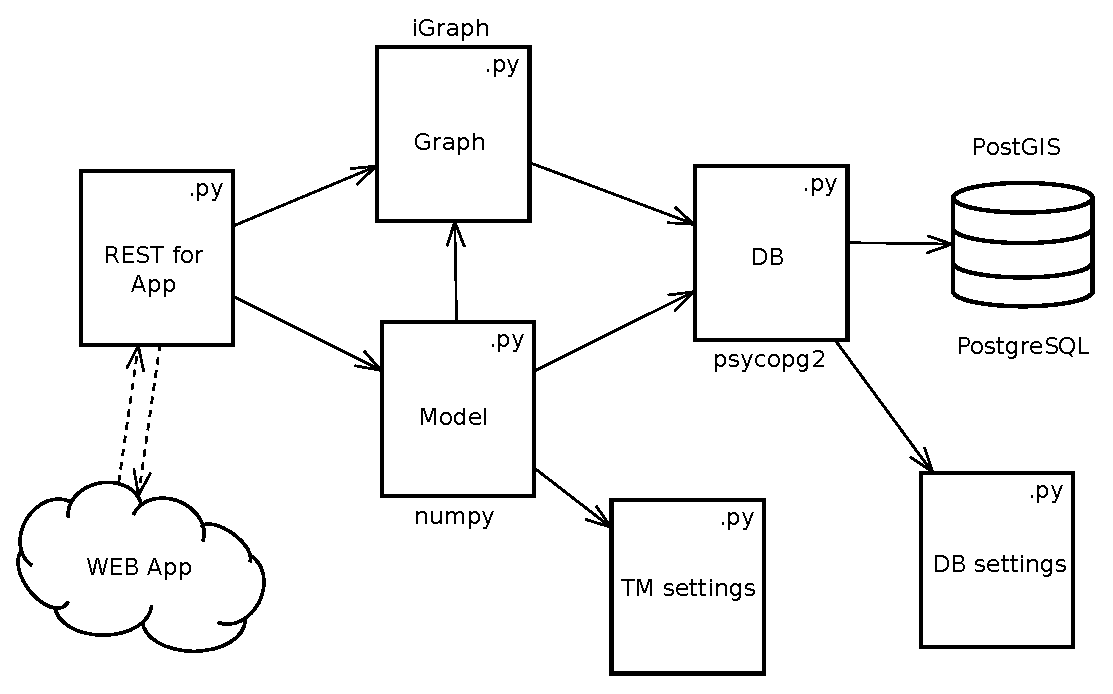
\includegraphics[width=15cm]{img/c01-transp-model/backend.eps}
\caption{Backend (REST)}
\label{img.b}
\end{figure}

Recompute traffic take a lot of time, so REST must be asynchronous. In our approach we made two service. First service start compute and second return progress.

Example:
\begin{verbatim}
/api/compute_traffic

{"status": "ok", "result": "calculation began"}

/api/compute_traffic_progress

{"status": "ok", "result": {"progress": 34, "isrun": true}}
\end{verbatim}

\chapter{Merge}
% MERGE - Data
%%%%%%%%%%%%%%%%%%%%%%%%%%%%%%%%%%%%%%%%%%%%%

% FR
%Cette dernière partie permet de faire le liant entre le modèle de transport calculé dans le premier paragraphe et l'application développée dans le second paragraphe. L'objectif final étant de visualiser les informations des habitudes de transport à vélo dans la ville de Hyvinkää au travers un navigateur web. Pour ce faire, nous nous appuierons sur les notions expliqués dans les paragraphes précédents : le modèle de transport aquis et calculé, l'application développée et configurée.

% EN
This last part allows for the binder between the transport model calculated in the first paragraph and the application developed in the second paragraph. The ultimate goal is to view information bicycle transportation habits in the city of Hyvinkää through a web browser. 

To do this, we will build on the concepts explained in the preceding paragraphs: the transport model acquired and calculated, the application developed and configured.

%%%%%%%%%%%%%%%%%%%%%%%%%%%%%%%%%%%%%%%%%%%%%%%%%%%%%%%%%%%%%%%%%%%%%%%%%
% FR
%\section{Services REST}

% EN
\section{REST Services}

% FR
% Pour que l'application puisse interagir avec le serveur, nous avons besoin de services REST expliqué dans le chapitre 2. Le script Python exécuté en Deamon sur le serveur propose des services REST. Chaque service est appellé par une requête HTTP depuis l'application puis retourne un JSON contenant les données demandées.

% EN

For the application to interact with the server, we need REST services described in chapter 2. The Python script running on the server in Deamon offers REST services. Each service is called by an HTTP request from the application and returns a JSON containing the requested data.

This service is based on python micro-framework Flask. Backend environment you can see in Fig. \ref{img.asas}
\begin{figure}
\centering
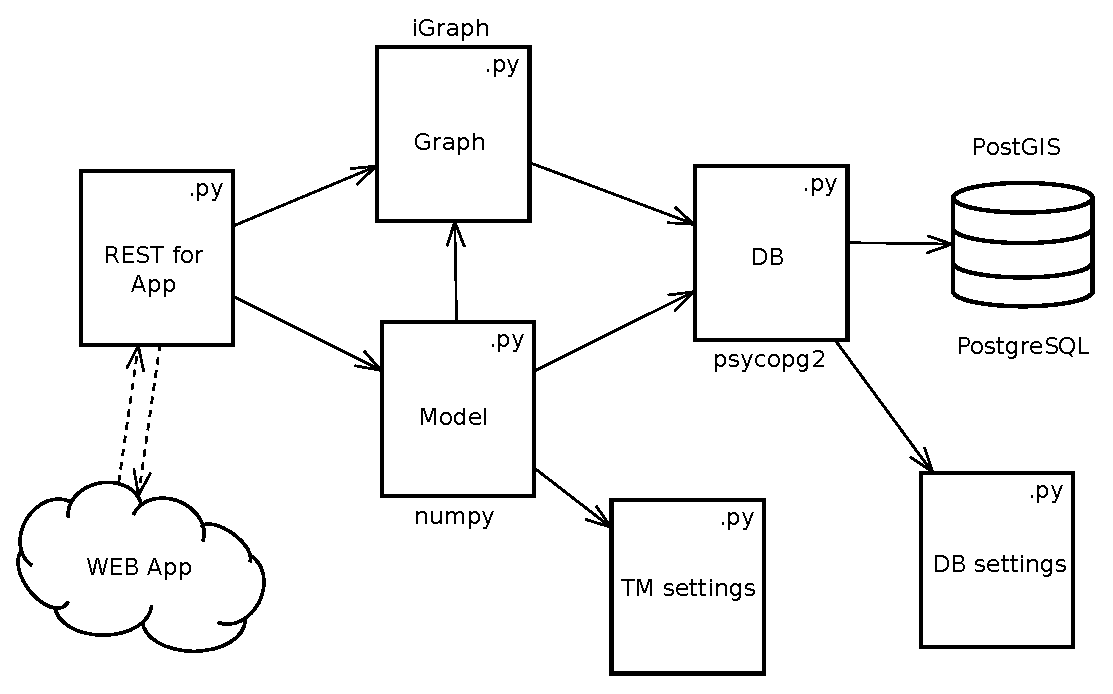
\includegraphics[width=15cm]{img/c01-transp-model/backend.eps}
\caption{Backend (REST)}
\label{img.asas}
\end{figure}

% FR
% La suite de ce paragraphe décrit chacun des services nécessaires et utilisés par l'application et explique les formats de JSON retournés.

% EN
The rest of this section describes each of the necessary services and used by the application and explains returned JSON formats.

\begin{description}

  \item[/api] \hfill \\ 
    Return an HTML list of all services on the REST API, with an example. \\
    \begin{lstlisting}[language=html]
<h2>Api info for TraMap</h2>
<ul>
  <li><b>/api/interests</b> - return type for tables (don't need any parameters)</li>
  <li><b>/api/ssp</b> - return Shortest path from A to B e.g
    <a href="api/ssp?lon1=24.87078&lat1=60.61663&lon2=24.85747&lat2=60.63003">
        api/ssp?lon1=24.87078&lat1=60.61663&lon2=24.85747&lat2=60.63003
    </a></li>
  <li><b>/api/compute_traffic</b> - start compute traffic (return info about start compute)</li>
  <li><b>/api/compute_traffic_progress</b> - progress for compute traffic</li>
<ul>
    \end{lstlisting}   
  \item[/api/interests] \hfill \\ 
    Return a JSON object with all the interests point by table. \\
    \begin{lstlisting}[language=javascript]
  {
    "status" : "ok",
    "result" : [
      {
        "table" : "roads",
        "interests" : [
          "motorway",
          "footway",
          "cycleway",
          "..."
        ]
      },{...}
    ]
  }
    \end{lstlisting} 
    
  \item[/api/ssp] \hfill \\ 
  
    Return a JSON object with the geometry shortest path, 
    time (in seconds) and distance (in meters) \\
    \begin{lstlisting}[language=javascript]
  {
    "status":"ok",
    "result":{
      "distance":1941.2000656999999,
      "features":[
        {
          "type":"LineString",
          "coordinates":[
          [
            24.8714912,
            60.6171716
          ],
          [
            24.8706363,
            60.6168433
          ],
          [
            24.870383,
            60.6167319
            ]
          ]
        },
        {...}
      ]
    }
  }
    \end{lstlisting}
    
  \item[/api/compute\_traffic] \hfill \\ 
  Recompute traffic take a lot of time, so REST must be asynchronous. In our approach we made two service. First service start compute and second return progress.  
    If you call this service, server start recomputing traffic and return information about start of recompute. \\
    \begin{lstlisting}[language=javascript]
{
"status": "ok",
"result": "calculation began"
}
    \end{lstlisting}
    
  \item[/api/compute\_traffic\_progress] \hfill \\ 
    This service is for view progress of recomputing traffic. Service return progress in \%.\\
    \begin{lstlisting}[language=javascript]
{
"status": "ok",
 "result": {
 			"progress": 34,
 			"isrun": true
 		   }
}
    \end{lstlisting}
  
\end{description}

% \begin{figure}[h]
%   \centering
%   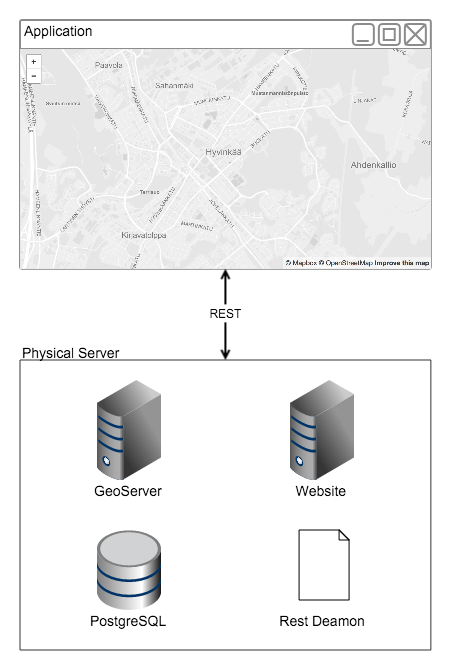
\includegraphics[width=8cm]{img/c02-application/png/app-server-interact.png}
%   \caption{Interaction between the application and the server}
% \end{figure}



% MERGE - App-Model
%%%%%%%%%%%%%%%%%%%%%%%%%%%%%%%%%%%%%%%%%%%%%


% MERGE
% ----------------------------------------------
\begin{figure}[ht]
    \centering
    \begin{subfigure}[b]{0.6\textwidth}
        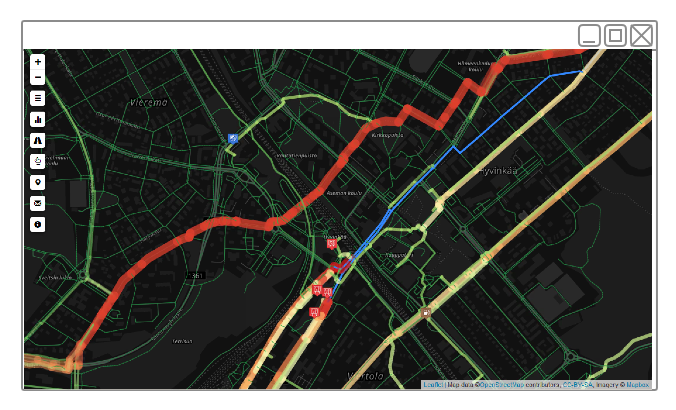
\includegraphics[width=\textwidth]
          {img/c03-merge/png/web-basemap-merge.png}
        \caption{Web}
    \end{subfigure}
    ~
    \begin{subfigure}[b]{0.2\textwidth}
        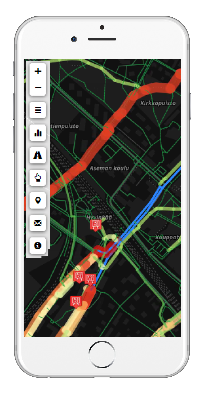
\includegraphics[width=\textwidth]
          {img/c03-merge/png/mobile-basemap-merge.png}
        \caption{Mobile}
    \end{subfigure}
    \caption{Application: Focus}
\end{figure}

\chapter*{Conclusion}
\addcontentsline{toc}{chapter}{Introduction}
% CONCLUSION
%%%%%%%%%%%%%%%%%%%%%%%%%%%%%%%%%%%%%%%%%%%%%

% FR
% L'information représente un actif important lié aux systèmes d'information géographique, dans le contexte actuel, la concurrence effrénée à laquelle se livrent les entreprises entraîne la multiplication des SIG comme atout majeur lors des décisions stratégiques.

% EN
Information is an important asset related to geographic information systems, in the current context, the unbridled competition that companies indulge causes the proliferation of GIS as a major asset in strategic decisions.

We done web application about transport information for Finland data source. Demo area is for city Hyvinkää in south Finland. Application is focused on bike traffic visualization with some additional function as finding shortest path.

Our solution can split to 2 part frontend and backend. Frontend is written in JavaScript using Leaflet. Backend is written in python using Python, Flask.

% FR


% EN










% BIBLIOGRAPHIE
%--------------------------------------
% TODO: Bibliography
\begin{thebibliography}{ABC}

    \bibitem[REF] {DocArcGIS} 
        \url{http://resources.arcgis.com/fr/help/}\\
        \emph{ArcGIS 10.3 Documentation}. 
        Environmental Systems Research Institute, Inc, 
        2015.

\end{thebibliography}

% ANNEXES
%--------------------------------------
\appendix

\newpage

%%%%%%%%%%%%%%%%%%%%%%%%%%%%%%%%%%%%%%%%%%%%%

\setlength{\parskip}{0em}
\listoffigures
\listoftables

% GLOSSAIRE
%--------------------------------------

\addcontentsline{toc}{chapter}{Glossaire}
\printglossaries

\end{document}